\documentclass{article}
\usepackage[utf8]{inputenc}
\usepackage{amsmath,amssymb}
\usepackage[letterpaper,margin=1in]{geometry}
\usepackage{graphicx,booktabs,array}
\usepackage[section]{placeins}
\usepackage{xcolor}
\usepackage{listings}
\usepackage{microtype,etoolbox}
\usepackage[font=small,labelfont=bf]{caption}
\usepackage{xurl}
\usepackage{hyperref}
\definecolor{reportblue}{HTML}{204E70}
\definecolor{reportgreen}{HTML}{386B59}
\hypersetup{hidelinks,
  pdftitle={AE 370 Group Project 1: Vertical Rocket Ascent},pdfauthor={Group 18}}
\setlength{\textfloatsep}{13pt plus 2pt minus 2pt}
\setlength{\intextsep}{12pt plus 2pt minus 2pt}
\renewcommand{\arraystretch}{1.12}
\pagestyle{plain}
\raggedbottom
\lstset{language=Python,basicstyle=\ttfamily\scriptsize,
  keywordstyle=\color{reportblue}\bfseries,commentstyle=\color{reportgreen},
  stringstyle=\color{reportblue},frame=single,rulecolor=\color{black!20},
  backgroundcolor=\color{black!2},breaklines=true,breakatwhitespace=false,
  numbers=left,numberstyle=\tiny\color{black!50},numbersep=6pt,
  showstringspaces=false,showspaces=false,showtabs=false,
  columns=fullflexible,keepspaces=true,tabsize=4,
  xleftmargin=1.5em,framexleftmargin=.4em,aboveskip=8pt,belowskip=8pt}
% Project repository URL.
\newcommand{\repositoryurl}{https://github.com/justinchiang0207/AE370-Sounding-Rocket-Ascent---Initial-Value-Problem}
\newcommand{\repositorylink}{\expandafter\url\expandafter{\repositoryurl}}
\makeatletter\newcommand{\inputrows}[1]{\@@input #1 }\makeatother
\begin{document}
\begin{titlepage}
    \centering % Centers the content on the page
    \vspace*{1cm} % Adds vertical space from the top of the page
    {\Huge\textbf{AE 370 Group Project 1}\par} % Title with large, bold font, followed by paragraph break
    \vspace{2cm} % Space between title and authors
    {\Large
        Maria Dalton \\ % Manual line break
        Morgan Waller \\ % Manual line break
        Yogeshwari Kant \\ % Manual line break
        Justin Chiang\par % Last line followed by paragraph break
    }
    \vspace{1cm} % Space between authors and group name
    {\large
        \textbf{Group 18} \\
        Aerospace Engineering, University of Illinois Urbana-Champaign
    }
    \vfill % Fills the remaining vertical space
    {\large Oct 28, 2026 \par} % Date at the bottom

\end{titlepage}

\section{The premise}
\subsection{Framing the Question}
The objective of this project is to investigate how rocket motor burn duration and propellant mass fraction affect the maximum altitude achieved by a vertically launched sounding rocket. Its maximum altitude depends on factors such as motor burn duration, propellant mass, gravitational forces, and aerodynamic drag. Increasing propellant mass changes the rocket's initial mass and mass depletion rate; whether it also increases impulse depends on the specified thrust and burn duration. Additionally, higher ascent velocities can increase aerodynamic drag and therefore reduce the altitude achieved. The engineering question we aim to investigate is: How do rocket motor burn duration and propellant mass fraction influence the maximum apogee altitude of a vertically launched sounding rocket, and how much does atmospheric drag reduce apogee for each motor configuration?
For the parameter studies, thrust $T_0$, dry mass, geometry, and environmental parameters are held fixed at their Table~\ref{tab:parameters} values. Define the propellant mass fraction by
\[
\phi=\frac{m_p}{m_0},\qquad m_0=\frac{m_{\mathrm{dry}}}{1-\phi},\qquad
m_p=m_0-m_{\mathrm{dry}},\qquad \dot m=\frac{m_p}{t_{\mathrm{burn}}}.
\]
Varying burn duration at fixed thrust changes total impulse $I=T_0t_{\mathrm{burn}}$. Varying $\phi$ at fixed thrust and burn duration changes mass, but not impulse. These are independent model-sensitivity studies, not comparisons of motors with a fixed specific impulse. The implied effective exhaust velocity $T_0/\dot m$ can vary between configurations. The drag penalty is defined by $h_{\mathrm{ap}}(C_d=0)-h_{\mathrm{ap}}(C_d=0.45)$ for otherwise identical parameters. Only immediate-lift-off configurations with $T_0>m_0g$ are considered; ground contact and delayed lift-off are not modeled.

\subsection{Relationship with Initial Value Problem}
In order to accurately predict the flight trajectory of the sounding rocket, multiple parameters must be considered. The acceleration of the rocket would be dependent on the following parameters:
\[\text{Signed aerodynamic resistance: }D\left(v,h\right)  = \frac{1}{2} \rho \left(h \right) v|v| C_d A\]
\[\text{Thrust: } T\left(t\right) = \begin{cases}
    T_0 & \text{if } 0\leq t < t_{burn} \\
    0  & \text{if } t \geq t_{burn} \end{cases} \]
\[\text{Mass: } m\left(t\right)  = \begin{cases}
    m_0 -\dot{m}t & \text{if } 0\leq t < t_{burn} \\
    m_\text{dry}  & \text{if } t \geq t_{burn} \end{cases} \]
We will need to incorporate atmospheric drag into our problem by using the following equations: 
Atmospheric density equation: 
\[\displaystyle \rho\left( h\right ) = \rho_0 e^{-h/H}\]
Substituting atmospheric density into drag:
\[D\left(v,h\right)  = \frac{1}{2} \left( \rho_0 e^{-h/H} \right) v|v| C_d A\]

\subsubsection{Equations Combined}
\[\boxed{\frac{dh}{dt} = v}\]
\[\boxed{\frac{dv}{dt} = \frac{T\left(t\right)}{m\left(t\right)}-g - \frac{\rho_0 C_d A}{2m\left(t\right)}\cdot e^{-h/H}v|v|}\]

\subsubsection{Initial Conditions}
\[h(0) = 0,\text{ } v(0) = 0,\text{ } m(0)=m_0\]
An Initial Value Problem (IVP) is necessary for this project because it allows us to predict the rocket's altitude and velocity over time using known starting conditions. The rocket's motion is constantly changing due to thrust, decreasing mass, gravity, and atmospheric drag. Since these factors make the governing differential equations difficult to solve analytically, we use a numerical method such as fourth-order Runge-Kutta (RK4) to approximate the rocket's trajectory. By solving the IVP, we can determine the rocket's maximum altitude (apogee) and analyze how burn duration and propellant mass affect its performance.
\subsection{Reason for Numerical Methods}
From the governing equations, it is evident that the terms are highly coupled, non-linear, and piecewise. The acceleration, $\dfrac{dv}{dt}$, depends on the drag, thrust, and mass of the rocket. Because velocity determines the altitude $h$, and altitude dictates the atmospheric air density, the drag force relies simultaneously on the exact integral of velocity (altitude) and the square of the velocity itself. These dependencies couple the two state equations. No closed-form solution for the full model is established here; numerical integration provides a practical way to evaluate its trajectories across the parameter study. Furthermore, the mass of the rocket decreases dynamically as propellant is consumed, and the thrust acts as a piecewise function that abruptly drops to zero at burnout.

We therefore use numerical methods to simulate the full trajectory, reserving analytically solvable special cases for verification. By defining the starting state, an Initial Value Problem is established. A numerical solver uses these initial conditions to evaluate acceleration at successive stage states. This iteratively approximates the instantaneous velocity, altitude, and drag as the rocket ascends.

\subsection{Mathematical Functions and Parameters}
The vertical flight of the sounding rocket is formulated as a second-order initial value problem expressed as a coupled system of first-order ordinary differential equations in state-space form:
\begin{equation}
    \mathbf{y}(t) = \begin{bmatrix} h(t) \\ v(t) \end{bmatrix}, \quad \frac{d\mathbf{y}}{dt} = \mathbf{f}(t, \mathbf{y})= \begin{bmatrix} f_1(t, h, v) \\ f_2(t, h, v) \end{bmatrix}
\end{equation}
where $h(t)$ is the vertical altitude and $v(t)$ is the vertical flight velocity.
\subsection{Auxiliary Models and Assumptions}
Thrust already represents the propulsive momentum flux. Thus the variable-mass equation is $m\dot v=T-D-mg$; adding a separate $-\dot m_{\mathrm{state}}v$ force would double-count the mass-flow effect in this thrust convention. During ascent $D\geq0$, so $-D$ opposes upward motion. The exponential atmosphere approximates an isothermal atmosphere with constant gravity. The prescribed positive consumption rate is $\dot m=(m_0-m_{\mathrm{dry}})/t_{\mathrm{burn}}$.

The numerical implementation augments the state to $u=[h,v,m]^T$, with $\dot m_{\mathrm{state}}=-\dot m$ during powered flight and zero during coast. Here $\dot m>0$ denotes the prescribed propellant consumption rate, not the signed derivative of the mass state. Integrating this third equation gives the same piecewise $m(t)$ used above.

The model assumes vertical point-mass motion, no wind or lift, constant gravity, a constant drag coefficient and reference area, and constant thrust within the burn. The parameters are illustrative model inputs rather than calibrated measurements of a particular motor. Constant $C_d$ does not resolve changes with Mach number; numerical convergence therefore verifies the discretization, not the real-world fidelity of this simplified model.

\subsubsection{Problem Parameters}
The physical constants, vehicle parameters, and numerical parameters governing this investigation are summarized in Table~\ref{tab:parameters}.

\begin{table}[htbp]
\centering
\caption{Physical, vehicle, and numerical parameters for the sounding rocket simulation.}
\label{tab:parameters}
\begin{tabular}{llcc}
\hline
\textbf{Category} & \textbf{Parameter} & \textbf{Symbol} & \textbf{Value / Unit} \\ \hline
\textbf{Environment} & Sea-level air density & $\rho_0$ & $1.225\text{ kg/m}^3$ \\
 & Scale height & $H$ & $8500\text{ m}$ \\
 & Standard acceleration of gravity & $g$ & $9.81\text{ m/s}^2$ \\ \hline
\textbf{Rocket Geometry} & Cross-sectional reference area & $A$ & $0.0314\text{ m}^2$ \\
 & Aerodynamic drag coefficient & $C_d$ & $0.45$ \\ \hline
\textbf{Mass \& Propulsion} & Initial gross mass & $m_0$ & $50.0\text{ kg}$ \\
 & Dry mass & $m_{\text{dry}}$ & $20.0\text{ kg}$ \\
 & Nominal thrust magnitude & $T_0$ & $2500\text{ N}$ \\
 & Nominal burn duration & $t_{\text{burn}}$ & $10.0\text{ s}$ \\ \hline
\textbf{Numerical Integration} & Integration time step & $\Delta t$ & Variable ($\text{s}$) \\
 & Initial conditions & $(h_0, v_0)$ & $(0\text{ m}, 0\text{ m/s})$ \\ \hline
\end{tabular}
\end{table}

%----------------------------------------------------------------------------

\section{The method}

\subsection{Justification} %Maria

\subsubsection{IVP Justification}
The sounding rocket's ascent is modeled as an IVP because the trajectory can be determined from a known initial state and a system of differential equations. The initial conditions establish that the rocket will begin at ground level with zero vertical velocity. The equations of motion describe how the altitude and velocity will transform under the influence of thrust, gravity, and the aerodynamic drag. Propellant consumption changes rocket mass; gravity and aerodynamic drag enter the force balance. Because the governing equations are nonlinear and coupled, a numerical method is necessary to approximate the rocket's trajectory and determine its maximum altitude. 

\subsubsection{Justification for Fourth-order Runge-Kutta (RK4) method}

\paragraph{A. Accuracy}


RK4 is a fourth-order numerical method, meaning that it provides relatively accurate approximations even when using moderately sized time steps. 
RK4 is a good choice because it achieves fourth order global accuracy. This means that its global numerical error behaves as: 
\[\boxed{E_{\text{global}} = O(\Delta t^4)}\]

This means that as we make the time step smaller, the numerical error decreases very quickly. 
This is especially important when calculating apogee, since it occurs when the rocket's upward velocity reaches zero. RK4 provides a reliable way to predict this point without requiring extremely small time steps, as long as we handle engine burnout correctly and verify time-step convergence. 

\paragraph{B. Stability}
The rocket's governing differential equations are:
\[\frac{dh}{dt} = v\]
\[\frac{dv}{dt} = \frac{T(t)}{m(t)} - g - \frac{\rho_0 C_d A}{2m(t)} e^{-h/H}v|v|\]

During each flight phase, the governing equations change smoothly as altitude, velocity, and mass change.  For typical sounding rocket parameters, we expect this system to be non-stiff, meaning that its dynamics do not require extremely small time steps solely to maintain numerical stability within each smooth flight phase. Smoothness alone does not establish non-stiffness; the local stability and step-refinement checks below assess this choice. Because of this, an explicit method like RK4 is a reasonable choice. 

\paragraph{C. Cost}
RK4 evaluates the differential equations four times during each step:
\[\boxed{\mathbf{y}_1,\ \mathbf{y}_2,\ \mathbf{y}_3,\ \mathbf{y}_4}\]
These four evaluations are combined to calculate the next altitude, velocity, and mass. By comparison, Euler's method only requires one evaluation per time step. At first, this might make RK4 seem more expensive. However, RK4 typically provides much higher accuracy at a given time step size, which can allow us to use fewer time steps to achieve a desired level of accuracy. 


RK4 is an explicit method, meaning that it calculates the next state directly from the current state. It does not require matrix inversion or solving nonlinear algebraic systems during each step. For our relatively small, non-stiff system, this makes RK4 a practical computationally efficient choice. 

%---------------------------------------------------------------------------

\subsection{The Mathematical Derivation and Properties} %Morgan & Justin

\subsubsection{Taylor-Series Foundation}%Justin
The Runge-Kutta 4th Order method is a numerical method that is meant to match the accuracy of a fourth-order Taylor series expansion without the calculation of complex higher order analytical derivatives. For an initial value problem that is defined as $\dfrac{du}{dt} = f\left(u,t\right)$, the Taylor series expansion of the state at the next time step $t_{k+1}=t_k + \Delta t $

\[u(t_{k+1}) = u(t_k) + \Delta t u'(t_k) + \frac{\Delta t^2}{2!} u''(t_k) + \frac{\Delta t^3}{3!} u'''(t_k) + \frac{\Delta t^4}{4!} u^{(4)}(t_k) + \mathcal{O}(\Delta t^5)\]

For a coupled, non-linear dynamical system, just like the problem discussed in this report, it is computationally expensive and complex deriving and evaluating these higher-order analytical derivatives $u''$, $u'''$, $u''''$. The Runge-Kutta 4th Order method avoids these derivative evaluations by evaluating the first derivative of the function $f(u,t)$ at four stage states within each time step $\left(t_{k} \text{ to } t_{k+1} \right)$. Then, the Runge-Kutta 4th Order method would perfectly match the coefficient of the Taylor series up to the $\Delta t^4$ term by using the weighted average of the 4 evaluations at four stage states (three distinct times). This makes the truncation error at that interval $\mathcal{O}(\Delta t^5)$ every step, with a global truncation error of $\mathcal{O}(\Delta t^4)$ for the entire simulation.

\subsubsection{Four Slopes}%Justin
Following Lecture~10, the Runge-Kutta 4th Order method evaluates $u(t_{k+1})$ from $u(t_k)$ using a weighted average of the governing differential equation evaluated at four different locations within the time step ($t_k$ to $t_{k+1}$). These evaluations, denoted as $y_1, y_2, y_3$, and $y_4$, represent the calculated slopes of the state trajectory at specific points. 

\paragraph{The first slope $y_1$:}
The first slope or rate of change is calculated based on the governing differential equation $f$ that defines how the system changes over time at the known location $u_k$ at time $t = t_k$. Therefore, $y_1$ can be expressed as:
\[y_1 = f(u_k, t_k)\]

\paragraph{The second slope $y_2$:}
The second slope or rate of change is calculated at the location of the midpoint between $t_k$ and $t_{k+1}$, which could be written as $t = t_k + \frac{1}{2}\Delta t$, based on the governing differential equation $f$. The estimated location at this midpoint used to calculate the rate of change is found by taking the known location $u_k$ and projecting it forward by half a time step using the initial slope $y_1$. Therefore, $y_2$ can be expressed as:
\[y_2 = f\left(u_k + \frac{1}{2}\Delta t y_1, t_k + \frac{1}{2}\Delta t\right)\]

\paragraph{The third slope $y_3$:}
The third slope or rate of change is calculated at the exact same midpoint $t=t_k + \frac{1}{2}\Delta t$, based on the governing differential equation $f$. However, instead of projecting forward using the initial slope, this calculation estimates the midpoint state by projecting the known location $u_k$ forward by half a time step using the newly calculated first midpoint slope $y_2$. Therefore, $y_3$ can be expressed as:
\[y_3 = f\left(u_k + \frac{1}{2}\Delta t y_2, t_k + \frac{1}{2}\Delta t\right)\]

\paragraph{The fourth slope $y_4$:}
The fourth slope or rate of change is calculated at the endpoint $t=t_k + \Delta t$, based on the governing differential equation $f$. The estimated location at this endpoint is determined by taking the known location $u_k$ and projecting it forward a full time step $\Delta t$ using the refined second midpoint slope $y_3$. Therefore, $y_4$ can be expressed as:
\[y_4 = f\left(u_k + \Delta t y_3, t_k + \Delta t\right)\]

\paragraph{The final equation:}
The final advanced location of the system is calculated by adding the product of the time step and the weighted average of the four previously evaluated slopes to the known location $u_k$. The specific weights are $\dfrac{1}{6}$, $\dfrac{2}{6}$, $\dfrac{2}{6}$, and $\dfrac{1}{6}$. 



The weights are selected together with the stage coefficients to match the exact solution's Taylor expansion through fourth order. They are not based on a general claim that midpoint values are more representative. The resulting update is
\[
u_{k+1}=u_k+\frac{\Delta t}{6}(y_1+2y_2+2y_3+y_4).
\]
To make the coefficient matching explicit, define the stage matrix $B$, weight vector $b$, and stage-time vector $c$:
\[
B=\begin{bmatrix}0&0&0&0\\ \tfrac12&0&0&0\\0&\tfrac12&0&0\\0&0&1&0\end{bmatrix},\quad
b=\begin{bmatrix}1/6\\1/3\\1/3\\1/6\end{bmatrix},\quad
c=B\mathbf{1}=\begin{bmatrix}0\\1/2\\1/2\\1\end{bmatrix}.
\]
Taylor-expanding each stage about the exact starting state and matching the independent derivative terms gives the following conditions through order four. This coefficient check supplements the RK4 formula in Lecture~10; $c^j$ denotes componentwise powers and $C=\operatorname{diag}(c)$:
\[
\begin{array}{c|l}
\text{Order}&\text{Conditions verified by these coefficients}\\\hline
1&b^T\mathbf{1}=1\\
2&b^Tc=1/2\\
3&b^Tc^2=1/3,\quad b^TBc=1/6\\
4&b^Tc^3=1/4,\quad b^TCBc=1/8,\quad b^TBc^2=1/12,\quad b^TB^2c=1/24
\end{array}
\]
For example, $Bc=(0,0,1/4,1/2)^T$, giving $b^TBc=1/12+1/12=1/6$, while $B^2c=(0,0,0,1/4)^T$, giving $b^TB^2c=1/24$. These are the conditions arising from the nonlinear stage states, in addition to the quadrature moment conditions $b^Tc^j=1/(j+1)$. For explicit time dependence, the same argument applies after adding $t'=1$ to the state. Under sufficient smoothness, the first unmatched terms are of order $\Delta t^5$. Appendix~\ref{app:derivation} shows the derivative terms that these conditions match.

%----------------------------------------------------------------------------
%----------------------------------------------------------------------------
\subsubsection{Error}%Morgan

The classical fourth-order Runge--Kutta method matches the Taylor
series expansion of the exact solution through terms of order
$\Delta t^4$. Therefore, its \textbf{local truncation error}, defined
as the error introduced by one step starting from the exact state,
is fifth order:
\[
E_{\mathrm{local}} = O(\Delta t^5).
\]
Lecture~11 divides this one-step defect by $\Delta t$, so its normalized truncation error is
\[
\tau_k=E_{\mathrm{local}}/\Delta t=O(\Delta t^4).
\]
Over a fixed simulation interval, the number of steps is proportional
to $1/\Delta t$. Provided the governing equations are sufficiently
smooth and the integration remains stable, the accumulated
\textbf{global truncation error} is fourth order:
\[
E_{\mathrm{global}} = O(\Delta t^4).
\]
More explicitly, a Lipschitz bound on the one-step map gives
$\|e_{k+1}\|\leq(1+L\Delta t+O(\Delta t^2))\|e_k\|+C\Delta t^5$.
Summing the resulting geometric bound over a fixed interval yields
$\|e_N\|=O(\Delta t^4)$ for exact initial data. The constants depend on solution smoothness and the interval; the order is an asymptotic statement, not an error bound for an arbitrary step.

Consequently, halving the time step should reduce the global error
by approximately a factor of $2^4 = 16$ when truncation error
dominates.

The RK4 update approximates the integral of the governing
differential equation over one time step:
\[
u(t_{k+1}) = u(t_k)
+ \int_{t_k}^{t_{k+1}} f(u(t),t)\,dt.
\]
Its weights,
\[
\left(\frac{1}{6},\frac{2}{6},\frac{2}{6},\frac{1}{6}\right),
\]
mirror Simpson's Rule by emphasizing the midpoint of the interval.
The two midpoint contributions have a combined weight of $4/6$,
corresponding to Simpson's endpoint--midpoint--endpoint weights
of $(1/6,4/6,1/6)$. However, RK4 evaluates its two midpoint slopes
using different estimated states, so it is not generally identical
to applying Simpson's Rule to the exact trajectory.

For the rocket model, the smoothness assumptions apply separately
during powered ascent and coasting. Because thrust changes abruptly
at burnout, each integration step must remain within a single flight
phase. The solver ends a step exactly at burnout, uses the powered
equations throughout that step, and then restarts with the coast
equations. This avoids evaluating stages across the discontinuity
and supports the expected fourth-order accuracy.

\subsubsection{Stability}%Morgan

Numerical stability describes how perturbations, including roundoff
and previously introduced errors, propagate through successive time
steps. Applying RK4 to the linear test equation
\[
\frac{du}{dt} = \lambda u
\]
gives
\[
u_{k+1} = R(z)u_k,
\qquad z = \lambda\Delta t,
\]
where the amplification factor is
\[
R(z) = 1 + z + \frac{z^2}{2}
+ \frac{z^3}{6} + \frac{z^4}{24}.
\]
For a strictly decaying test mode, the interior of the absolute-stability region satisfies
\[
|R(\lambda\Delta t)| < 1.
\]
The equality $|R|=1$ describes the boundary and does not imply decay. Substituting $f=\lambda u$ into the stages gives $y_1=\lambda u_k$, $y_2=\lambda(1+z/2)u_k$, $y_3=\lambda(1+z/2+z^2/4)u_k$, and $y_4=\lambda(1+z+z^2/2+z^3/4)u_k$; their weighted sum yields the stated $R(z)$, following Lecture~12.

RK4 has a bounded stability region and is therefore conditionally
stable. An excessively large time step can cause numerical errors
to grow even when the corresponding physical mode decays.

For the nonlinear rocket equations, local stability can be assessed
using the eigenvalues of the Jacobian of the governing equations
within each flight phase. For the equivalent two-state formulation with prescribed $m(t)$, during ascent ($v\geq0$),
\[
J=\begin{bmatrix}0&1\\D/(mH)&-\rho C_dAv/m\end{bmatrix}.
\]
For the implemented three-state formulation, the mass column is
\[
[0,-(T-D)/m^2,0]^T.
\]
The third row is zero, introducing a zero eigenvalue. The two-state Jacobian has one positive and one negative eigenvalue when drag is nonzero and $v>0$: growth in a physical perturbation is not automatically numerical instability. Decaying modes should lie within RK4's
stability region after multiplication by $\Delta t$. Time-step
refinement is also needed to establish that the predicted trajectory
and apogee are sufficiently accurate, since numerical stability
alone does not guarantee accuracy.


%----------------------------------------------------------------------------

\subsection{Algorithmic Summary}%Yogeshwari
The logical execution flow of the custom RK4 simulation and apogee detection routine is structured into sequential steps, detailed below:

\begin{enumerate}
    \item \textbf{Initialization:} Set the initial simulation time to zero, load the vehicle parameters, and define the starting state vector containing initial altitude, velocity, and mass.
    \item \textbf{Main Time Loop:} Begin a loop that advances forward in time until the maximum simulation time is reached.
    \item \textbf{Burn Status and Time-Step Adjustment:} 
    \begin{itemize}
        \item Check if the current time is within the motor's active burn duration.
        \item Dynamically clip the time step size to ensure it does not exceed the remaining mission time or overshoot the exact instant of engine burnout.
    \end{itemize}
    \item \textbf{Fourth-Order Runge-Kutta (RK4) Evaluation:} 
    \begin{itemize}
        \item Compute the four intermediate slopes ($k_1, k_2, k_3, k_4$) by evaluating the governing equations of motion (incorporating atmospheric density, aerodynamic drag, thrust, and gravity) across the trial intervals.
        \item Advance the flight state using the standard weighted average of the four slopes multiplied by the time step.
        \item If engine burnout occurs within the current interval, explicitly enforce the final dry mass.
    \end{itemize}
    \item \textbf{Apogee Event Detection:} Monitor the vertical velocity across the step. If the velocity transitions from positive (climbing) to negative (falling), trigger a bisection root-finding routine to localize the numerical apogee, record the final apogee state, and terminate the simulation.
    \item \textbf{Data Logging and Progression:} Record the updated time and state vector into the history logs, advance the current time clock, and proceed to the next iteration if apogee has not yet been reached.
\end{enumerate}

%----------------------------------------------------------------------------
\section{Correct implementation}

\subsection{Core Solver Implementation}%Maria

\subsubsection{Explanation of Core Solver}

    The sounding rocket's equations of motion were implemented in Python using a fourth-order Runge-Kutta, RK4, numerical solver. The solver uses a state vector consisting of altitude, vertical velocity, and rocket mass. This allows for all three variables to be advanced simultaneously at each time step. A derivative function was used to evaluate the effects of thrust, gravity, aerodynamic drag, and propellant consumption. The RK4 implementation calculates four intermediate estimates in order to determine the next state. 
    To accurately represent the rocket's flight, the solver accounts for the transition between powered ascent and unpowered coasting. The time steps are adjusted to end exactly at the engine burnout. This ensures that the thrust and propellant mass loss are properly discontinued. The simulation continues until the vertical velocity reaches zero, which allows the maximum apogee altitude to be determined. 
    The implementation was verified by comparing the numerical results with the analytical solution for the simplified flight conditions. Additional convergence studies were performed using progressively smaller time steps to evaluate numerical accuracy and confirm the expected fourth-order convergence behavior. 

The complete source of \texttt{rocket\_solver.py} is printed directly from the executable file in Appendix~\ref{app:code}; the experiment scripts are supplied in the repository. 

The state is $(h,v,m)$ throughout every RK4 stage. All stages of a step ending at burnout use the powered equations, including the endpoint stage, which evaluates the left-hand limit. The next step uses the coast equations. The state is continuous at burnout, and resetting $m$ to the prescribed dry mass only removes floating-point drift from an exactly linear mass law.

When $v_k>0$ and $v_{k+1}\leq0$, 45 bisection iterations solve for a fractional RK4 step from the same left endpoint. This avoids identifying apogee with the largest sampled altitude. At a coasting apogee, $\dot v=-g\ne0$, so the root is simple: an $O(\Delta t^4)$ state error produces an $O(\Delta t^4)$ event-time error locally, provided the crossing is bracketed and root-finding error is smaller. Numerical runs reject a failed lift-off, a nonfinite state, or reaching the time limit without locating apogee.

\subsection{Convergence Rate Study}%Yogeshwari

To verify the mathematical correctness and implementation order of the custom 4th-order Runge-Kutta (RK4) solver, a numerical convergence study was performed. The global discretization error was evaluated by comparing simulation outputs against a high-precision reference solution computed using an extremely refined time step ($\Delta t_{\text{ref}} = 0.0005\,\text{s}$). 

The error $E$ as a function of time step size $\Delta t$ is modeled by the asymptotic power-law relation:
\begin{equation}
    E(\Delta t) \approx C (\Delta t)^p
\end{equation}
where $p$ represents the empirical convergence rate (the slope on a log-log error plot). For a pure, unconstrained 4th-order Runge-Kutta method applied to a smooth differential equation, the theoretical convergence rate is $p = 4.0$.

\subsubsection{Implementation}
\texttt{convergence\_study.py} evaluates a sequence of halved steps, compares each apogee with a refined numerical reference, computes adjacent-step orders, and fits the slope of $\log E$ against $\log\Delta t$. The independent analytical checks below are needed because self-convergence cannot detect a consistently incorrect differential equation.

\subsubsection{Results and Discussion}
The Table~\ref{tab:parameters} convergence study uses $\Delta t=1,0.5,0.25,0.125$ s, with a reference step of $0.0005$ s. The measured apogee errors are $7.87337\times10^{-2}$, $4.33276\times10^{-3}$, $2.53042\times10^{-4}$, and $1.52730\times10^{-5}$ m. The adjacent-step observed orders,
\[
p_{\mathrm{obs}}=\log_2\!\left(\frac{E(\Delta t)}{E(\Delta t/2)}\right),
\]
are $4.184$, $4.098$, and $4.050$, respectively; the fitted slope is approximately $4.109$. The trend toward four supports the expected RK4 order. Halving the reference step changes apogee by approximately $6.97\times10^{-9}$ m, well below the smallest error fitted here.

A fit extending into the floating-point/reference-error floor can give a misleading slope. Burnout does not inherently reduce the order here because all stages remain within their selected flight phase. The 45 bisection iterations reduce the event-time bracket to at most $\Delta t/2^{45}$ in exact arithmetic; integration and floating-point errors still remain. Convergence alone does not validate the governing equations, so independent checks follow.
\begin{figure}[htbp]
    \centering
    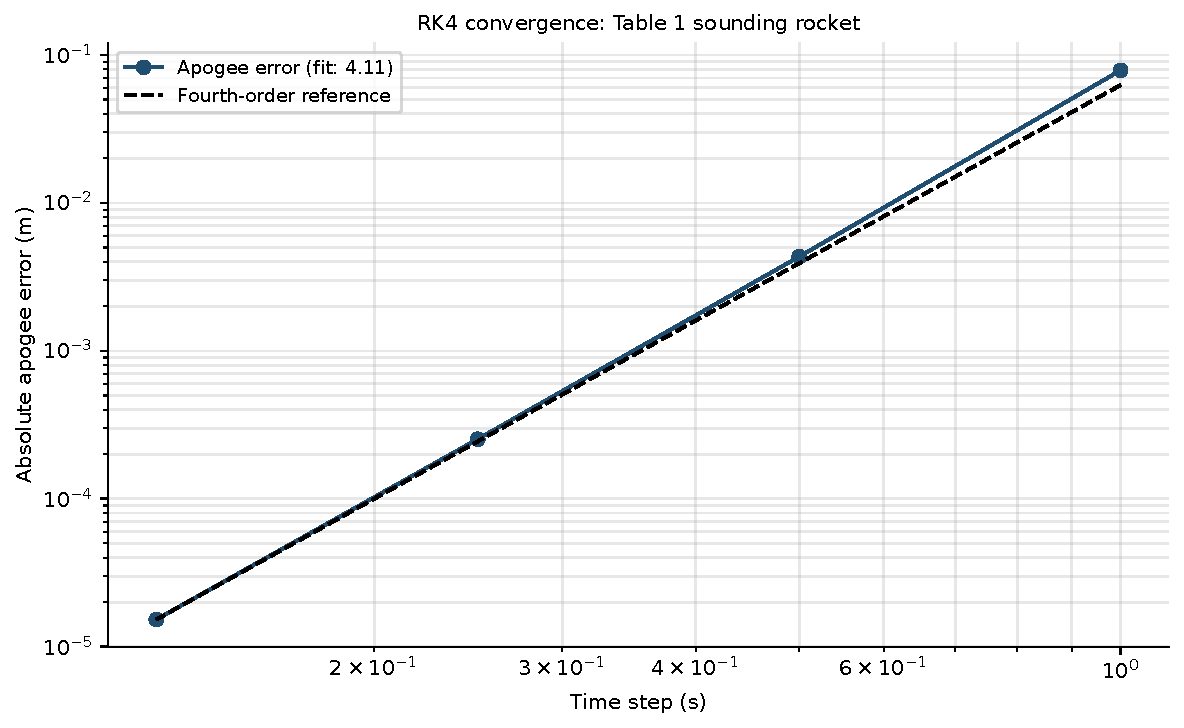
\includegraphics[width=0.75\linewidth]{figures/convergence.pdf}
    \caption{Apogee convergence for Table~\ref{tab:parameters}; adjacent-step orders approach four before the numerical error floor.}
    \label{fig:check4}
\end{figure}
%----------------------------------------------------------------------------
\subsection{Independent Analytical Validation}%Justin
While a standard error study (such as progressively halving the time step $\Delta t$) confirms that a numerical integration scheme converges at its theoretical rate, it is insufficient to prove the accuracy of the underlying physical model. A numerical solver will smoothly and predictably converge upon the solution of a fundamentally flawed differential equation—such as one with an inverted gravity vector or an incorrectly scaled mass flow rate. Therefore, to check that the solver evaluates the intended equations, its output is compared against a known, independent analytical solution. 

\subsubsection{Defining the Special Case Limit}
The full Initial Value Problem (IVP) governing the ascent of the sounding rocket is defined by a complex sum of forces, including thrust ($T$), non-linear aerodynamic drag ($D$), and gravity ($mg$):
\[ m \frac{dv}{dt} = T - \frac{1}{2}\rho v|v| C_d A - mg \]

Because air density ($\rho$) is a function of altitude and mass ($m$) varies with time during the engine burn, we use numerical integration for the full model. To create a mathematical benchmark, we isolate a special case limit where these complex terms drop out. By setting $C_d=0$, $T=0$, $t_{\mathrm{burn}}=0$, and $m_0=m_{\mathrm{dry}}=50$ kg, the system is reduced to a constant-mass projectile operating in a vacuum. The governing equation simplifies dramatically as the mass term cancels out:
\[ m \frac{dv}{dt} = -mg \implies \frac{dv}{dt} = -g \]

\subsubsection{The Analytical Benchmark}
By integrating this simplified linear limit with respect to time, the exact analytical solutions for velocity and altitude are derived as standard kinematic equations:
\[ v(t) = \int -g \, dt = v_0 - gt \]
\[ h(t) = \int (v_0 - gt) \, dt = h_0 + v_0 t - \frac{1}{2}gt^2 \]
These exact equations serve as an absolute baseline. If the Python implementation of the physics engine and the RK4 loops are constructed correctly, the numerical output for this simplified state should agree with these kinematic solutions to floating-point accuracy.

\subsubsection{Verification Execution and Analysis}
The custom Runge-Kutta 4th Order (RK4) solver was configured with these simplified parameters and initialized with a starting velocity of $v_0 = 150$ m/s from an altitude of $h_0 = 0$ m. The simulation was executed with a time step of $\Delta t = 0.1$ seconds. At each discrete time step, the numerical altitude and velocity states were subtracted from the exact analytical states to calculate the absolute error.

The theoretical local truncation error of the RK4 method is $\mathcal{O}(\Delta t^5)$, for sufficiently smooth systems. For this constant-acceleration system, direct substitution into the RK4 stages gives $v_{k+1}=v_k-g\Delta t$ and $h_{k+1}=h_k+v_k\Delta t-g\Delta t^2/2$. Because the exact analytical solution for altitude under constant acceleration is a quadratic polynomial (degree 2), the mathematical truncation error for this specific test case is exactly zero. Upon running the simulation, the maximum recorded discrepancy between the RK4 numerical altitude and the exact analytical altitude was approximately $4.77\times10^{-12}$ meters in the executed run. This small residual is consistent with accumulated floating-point roundoff; its absolute size depends on trajectory scale and the number of steps. 

\begin{figure}[htbp]
    \centering
    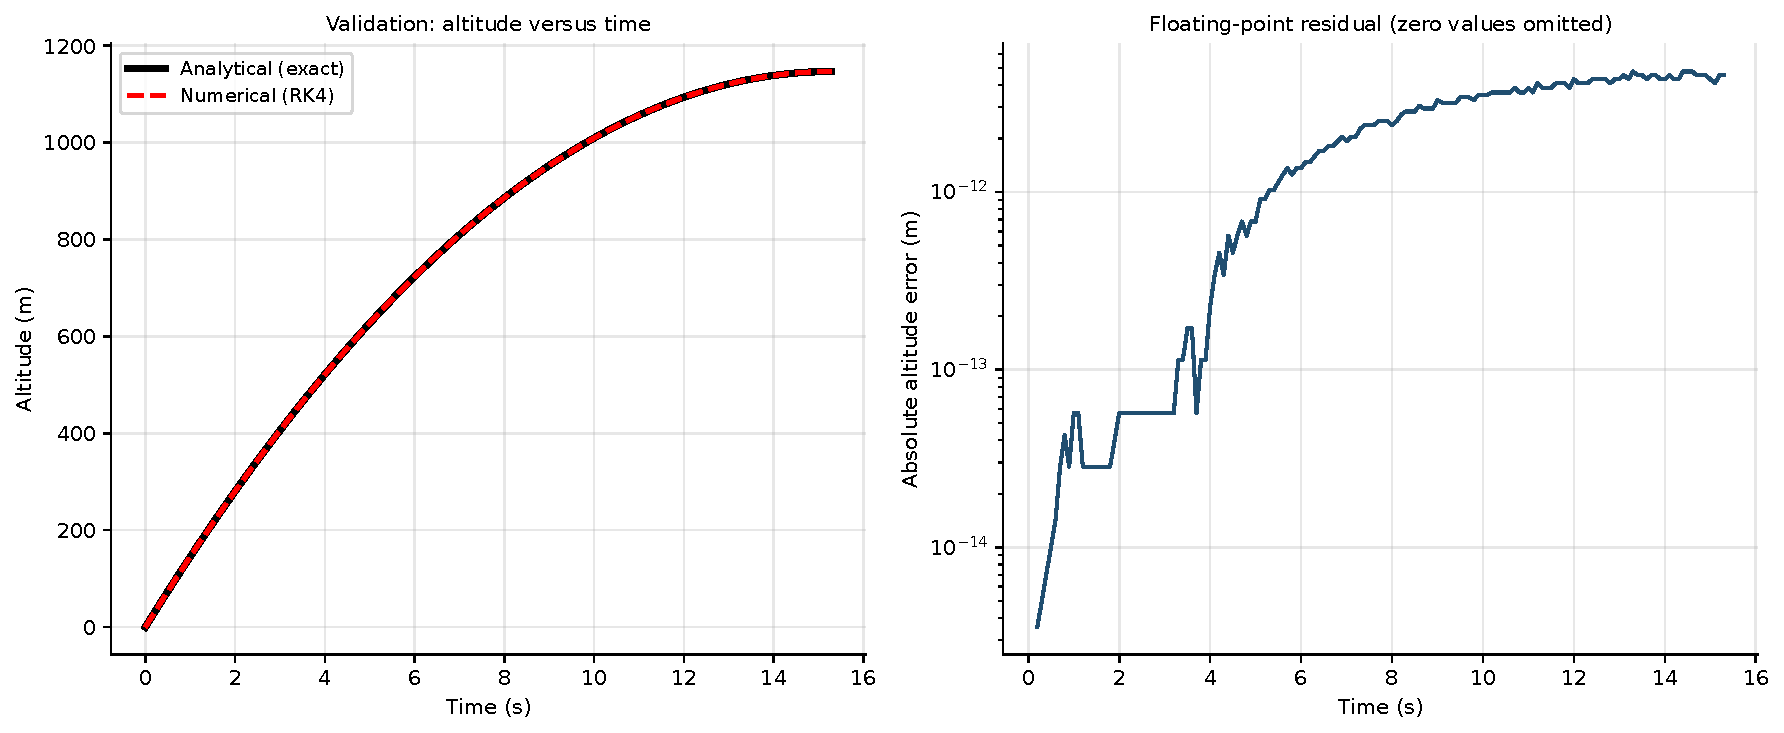
\includegraphics[width=1\linewidth]{figures/verification.pdf}
    \caption{Ballistic vacuum validation with $v_0=150$ m/s and $\Delta t=0.1$ s. Zero errors are omitted from the logarithmic error panel.}
    \label{fig:check5}
\end{figure}

This test checks constant-acceleration kinematics, state indexing, and apogee localization, but does not test thrust or drag because they are disabled. It is evidence for this special case, not a proof that every part of the solver is correct.

An additional independently derived check retains thrust and changing mass while setting $C_d=0$. During powered flight, let $q=\dot m>0$ and $m(t)=m_0-qt$. Integrating $\dot v=T_0/m(t)-g$ with $v(0)=h(0)=0$ gives
\[
v(t)=\frac{T_0}{q}\ln\frac{m_0}{m(t)}-gt,
\qquad
h(t)=\frac{T_0}{q^2}\left[m_0-m(t)-m(t)\ln\frac{m_0}{m(t)}\right]-\frac12gt^2.
\]
For example, $\int_0^t\ln[m_0/(m_0-qs)]\,ds=[m_0-m(t)-m(t)\ln(m_0/m(t))]/q$, giving the altitude expression. Both expressions satisfy the initial conditions and differentiate back to the drag-free equations. At burnout, the altitude errors for $\Delta t=0.5,0.25,0.125$ s are $3.5562\times10^{-4}$, $2.2283\times10^{-5}$, and $1.3936\times10^{-6}$ m, approximately a factor of 16 per halving. This checks powered variable-mass integration. Separate automated checks verify drag direction, the exponential density ratio, non-grid-aligned burnout, and failure handling. No comparison with measured flight data has been performed.

%----------------------------------------------------------------------------
\subsection{Simulation Parameter Evaluation}%Morgan

The time step must be small enough to accurately predict apogee while
remaining computationally efficient for repeated simulations of different
burn durations and propellant mass fractions. This evaluation uses the
physical parameters in Table~\ref{tab:parameters}, including
$m_0=50\,\mathrm{kg}$, $m_{\mathrm{dry}}=20\,\mathrm{kg}$,
$T_0=2500\,\mathrm{N}$, and $t_{\mathrm{burn}}=10\,\mathrm{s}$.
The corresponding propellant mass flow rate is
\[
\dot{m}=\frac{m_0-m_{\mathrm{dry}}}{t_{\mathrm{burn}}}
       =3\,\mathrm{kg/s}.
\]
For this evaluation, the numerical accuracy targets are chosen to be
$0.1\,\mathrm{m}$ in apogee altitude and $0.001\,\mathrm{s}$ in
apogee time, measured against a refined numerical reference.

\subsubsection{Acceleration Variation and Flight-Phase Transitions}

During ascent, the rocket's acceleration is
\[
a=\frac{T-D}{m}-g,
\qquad
D=\frac{1}{2}\rho(h)C_dAv^2.
\]
The rate of change of acceleration, or jerk, indicates how quickly the
dynamics vary. Let $q=-dm/dt$, so that $q=\dot{m}$ during powered
flight and $q=0$ during coast. Within either smooth flight phase,
differentiating the acceleration gives
\[
\frac{da}{dt}
=
\frac{q(T-D)}{m^2}
-\frac{\rho(h)C_dA}{m}va
+\frac{Dv}{mH}.
\]
These terms account for changing mass, velocity-dependent drag, and
decreasing atmospheric density, respectively.

The refined nominal simulation gives a maximum sampled jerk magnitude
of approximately $3.00\,\mathrm{m/s^3}$ during powered ascent. Immediately
after burnout, the jerk is approximately $28.95\,\mathrm{m/s^3}$.
Although the mass becomes constant during coast, the rocket initially
experiences strong aerodynamic deceleration. Therefore, a larger coast
time step cannot be justified solely by the absence of thrust; it must
be supported by a numerical accuracy comparison.

Burnout also introduces an instantaneous acceleration change:
\[
a(t_{\mathrm{burn}}^+)-a(t_{\mathrm{burn}}^-)
=-\frac{T_0}{m_{\mathrm{dry}}}
=-125\,\mathrm{m/s^2}.
\]
For the nominal trajectory, acceleration changes from approximately
$43.58\,\mathrm{m/s^2}$ to $-81.42\,\mathrm{m/s^2}$.
This discontinuity is handled by shortening the final powered step
to end exactly at $t_{\mathrm{burn}}$. All four RK4 stages of that
step use the powered equations, and the next step uses the coast
equations. Consequently, no RK4 step mixes the two flight phases.

\subsubsection{Time-Step Accuracy Study}

The existing RK4 algorithm was evaluated with independently selected
powered and coast time steps. All 25 combinations drawn from
\[
\Delta t_{\mathrm{powered}},\,
\Delta t_{\mathrm{coast}}
\in
\{0.1,\;0.25,\;0.5,\;1.0,\;2.0\}\,\mathrm{s}
\]
were tested. Each simulation retained exact burnout alignment and
the existing 45-iteration bisection procedure for locating the
numerical apogee event.

A uniform reference step of
$\Delta t_{\mathrm{ref}}=0.0005\,\mathrm{s}$ produced
\[
h_{\mathrm{ap,ref}}=5806.866708\,\mathrm{m},
\qquad
t_{\mathrm{ap,ref}}=32.958766812\,\mathrm{s}.
\]
Halving the reference step to $0.00025\,\mathrm{s}$ changed these
quantities by approximately $7.0\times10^{-9}\,\mathrm{m}$ and
$7.9\times10^{-11}\,\mathrm{s}$, respectively. These differences
are negligible relative to the chosen accuracy targets. The reference
is used to assess time-discretization error; it is not an independent
validation of the physical model.

The errors are defined as
\[
E_h=\left|h_{\mathrm{ap}}-h_{\mathrm{ap,ref}}\right|,
\qquad
E_t=\left|t_{\mathrm{ap}}-t_{\mathrm{ap,ref}}\right|.
\]
Representative results are presented in
Table~\ref{tab:simulation_parameter_evaluation}, where $N$ is the
number of main RK4 steps, including the step that brackets apogee.

\begin{table}[htbp]
\centering
\caption{Time-step accuracy and computational cost for the
Table~\ref{tab:parameters} rocket parameters.}
\label{tab:simulation_parameter_evaluation}
\small
\begin{tabular}{ccrrr}
\hline
$\Delta t_{\mathrm{powered}}$ &
$\Delta t_{\mathrm{coast}}$ &
$E_h$ & $E_t$ & $N$ \\
$(\mathrm{s})$ & $(\mathrm{s})$ &
$(\mathrm{m})$ & $(\mathrm{s})$ & \\
\hline
0.1 & 0.1 & $6.21\times10^{-6}$ & $8.07\times10^{-9}$ & 330 \\
0.1 & 0.5 & $3.67\times10^{-3}$ & $4.02\times10^{-6}$ & 146 \\
0.5 & 0.5 & $4.33\times10^{-3}$ & $6.03\times10^{-6}$ & 66 \\
0.5 & 1.0 & $6.79\times10^{-2}$ & $8.51\times10^{-5}$ & 43 \\
1.0 & 0.5 & $1.52\times10^{-2}$ & $3.95\times10^{-5}$ & 56 \\
1.0 & 1.0 & $7.87\times10^{-2}$ & $1.19\times10^{-4}$ & 33 \\
2.0 & 1.0 & $2.76\times10^{-1}$ & $7.44\times10^{-4}$ & 28 \\
1.0 & 2.0 & $1.37$             & $2.10\times10^{-3}$ & 22 \\
2.0 & 2.0 & $1.57$             & $2.73\times10^{-3}$ & 17 \\
\hline
\end{tabular}
\end{table}

Increasing the coast step from $0.5\,\mathrm{s}$ to
$1.0\,\mathrm{s}$ while retaining a powered step of
$0.5\,\mathrm{s}$ reduces the main step count from 66 to 43
while satisfying both accuracy targets. Increasing the powered
step to $1.0\,\mathrm{s}$ further reduces the count to 33.
However, assigning $2.0\,\mathrm{s}$ to either phase fails the
altitude tolerance for every tested combination.

A local stability check using the Jacobian of the governing equations
gives a most negative eigenvalue of approximately
$-0.333\,\mathrm{s^{-1}}$ along the nominal trajectory.
For $\Delta t=1.0\,\mathrm{s}$, the RK4 amplification factor for
this fastest decaying mode is approximately $0.717$, within the
method's absolute stability region. This local check supports the
selected step, while the refinement results establish its accuracy
for the quantities of interest.

\subsubsection{Selected Parameters and Application to the Results}

For the nominal Table~\ref{tab:parameters} case, the selected setting is
\[
\boxed{
\Delta t_{\mathrm{powered}}
=
\Delta t_{\mathrm{coast}}
=
1.0\,\mathrm{s}
}
\]
because it is the least expensive of the 25 tested combinations
that satisfies both prescribed tolerances. It predicts
\[
h_{\mathrm{ap}}=5806.787974\,\mathrm{m},
\qquad
t_{\mathrm{ap}}=32.958648254\,\mathrm{s}.
\]
Including apogee localization, this setting requires 316 derivative
evaluations, compared with 1504 for a uniform $0.1\,\mathrm{s}$
step, a reduction of approximately $79\%$. If greater numerical
margin is desired, a uniform $0.5\,\mathrm{s}$ step reduces the
apogee error to approximately $0.00433\,\mathrm{m}$.

The maximum simulation time remains $120\,\mathrm{s}$, which exceeds
the nominal apogee time. Integration terminates at the localized
zero-velocity event rather than selecting the largest sampled
altitude. Any simulation that reaches the time limit before this
event raises an error and must be extended rather than treating its final altitude
as apogee. Configurations that cannot lift off immediately are also rejected.

The $1$ s choice is specific to the nominal case. The Results study instead uses uniform $0.125$ s steps, with $0.5$ and $0.25$ s comparisons for every configuration. Both successive differences satisfy the same $0.1$ m and $0.001$ s criteria. The largest final-halving differences are $0.00264$ m and $1.63\times10^{-5}$ s; these are observed refinement differences, not certified exact-error bounds. A configuration-dependent time limit of $\max(120\,\mathrm{s},2t_{\mathrm{ap,vac}})$ permits the longer vacuum flights. All runs terminate at the apogee event. Detailed study controls and numerical safeguards are given in Section~4.

\section{Results}
\subsection{Study Design and Nominal Flight}
To study the effects of burn duration and propellant mass fraction, we used 21 burn durations ($5$--$15$ s in $0.5$ s increments) and 17 propellant fractions ($0.40$--$0.80$ in increments of $0.025$), for 357 configurations. This range brackets the nominal $(10\,\mathrm{s},0.60)$ case and probes both parameters without approaching the lift-off boundary. Thrust is fixed at $2500$ N, dry mass at $20$ kg, and all geometry and atmospheric quantities at Table~\ref{tab:parameters} values. The initial mass consequently ranges from $33.33$ to $100$ kg; even the heaviest case has $T_0/(m_0g)=2.55>1$.

Each atmospheric trajectory is integrated at $\Delta t=0.5$, $0.25$, and $0.125$ s. The finest trajectory supplies the reported results, while both successive refinements are checked against the selected altitude and time tolerances. Drag-free trajectories at $0.125$ s are independently compared with the exact powered-plus-coasting solution in Appendix~\ref{app:vacuum}. Across all 357 cases, the largest vacuum discrepancies are $6.27\times10^{-4}$ m in apogee and $3.30\times10^{-6}$ s in apogee time. The drag penalty uses the analytical vacuum apogee to avoid an additional numerical-reference error:
\begin{equation}
 \Delta h_D=h_{\mathrm{ap,vac}}-h_{\mathrm{ap,atm}},\qquad
 P_D=100\frac{\Delta h_D}{h_{\mathrm{ap,vac}}}\quad(\%).
 \label{eq:drag-penalty}
\end{equation}
This difference includes drag's effects during powered flight and coast. It is an altitude penalty between two complete trajectories, not a direct drag-work measurement.

For the nominal case, atmospheric apogee is $5806.87$ m at $32.95877$ s. Figure~\ref{fig:nominal} provides the trajectory context; the parameter comparisons that answer the engineering question follow in Figures~\ref{fig:slices}--\ref{fig:drag-results}. Mass decreases linearly to $20$ kg at $10$ s, remains constant thereafter, and upward velocity decreases to zero at apogee. The state is continuous at burnout even though acceleration jumps.
\begin{figure}[htbp]
\centering
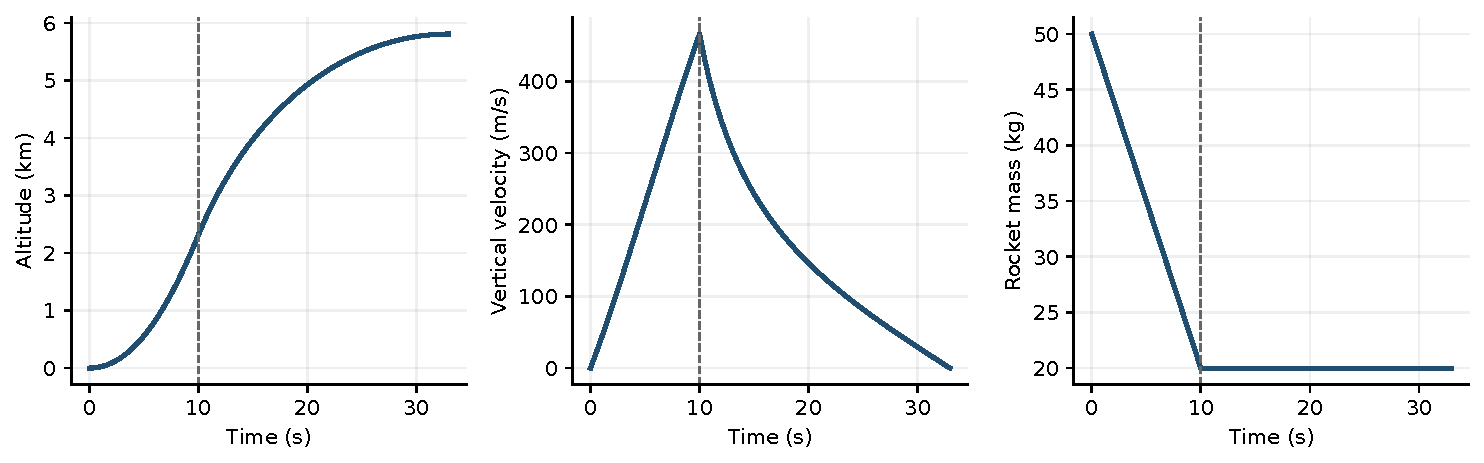
\includegraphics[width=\linewidth]{figures/nominal_trajectory.pdf}
\caption{Nominal atmospheric trajectory ($\phi=0.60$, $t_{\mathrm{burn}}=10$ s), plotted at $\Delta t=0.1$ s. Dashed lines mark burnout. The final point is the localized zero-velocity event.}
\label{fig:nominal}
\end{figure}

\subsection{Effect of Motor Burn Duration}
At every sampled propellant fraction, atmospheric apogee increases with burn duration. For the nominal fraction $\phi=0.60$, increasing the duration from $5$ to $10$ to $15$ s gives $2613.40$, $5806.87$, and $9669.68$ m, respectively. The $15$ s case reaches approximately $3.70$ times the altitude of the $5$ s case. The smallest altitude gain between adjacent $0.5$ s duration samples anywhere on the grid is $209.80$ m, far larger than the observed refinement changes.

This trend follows from the specified comparison: at fixed thrust, impulse increases from $12{,}500$ to $37{,}500$ N\,s as the burn is lengthened. At fixed propellant fraction the propellant mass stays constant, so a longer burn also lowers the mass-flow rate and increases the implied effective exhaust velocity $T_0/\dot m$. The result therefore does not isolate a burn-time effect at fixed impulse or fixed exhaust velocity.

The exact constant-gravity vacuum solution has $h_{\mathrm{ap,vac}}\propto t_{\mathrm{burn}}^2$ at a fixed propellant fraction (Appendix~\ref{app:vacuum}). The atmospheric case does not follow that simple scaling because drag couples altitude, density, and velocity. Near the nominal case, a centered difference using the $9.5$ and $10.5$ s runs gives
\[
 \left.\frac{\partial h_{\mathrm{ap}}}{\partial t_{\mathrm{burn}}}\right|_{\phi=0.6,t_{\mathrm{burn}}=10\,\mathrm{s}}
 \approx 686.89\ \mathrm{m/s}.
\]
This is a finite-difference sensitivity over the stated spacing, not a universally constant slope.

\subsection{Effect of Propellant Mass Fraction}
At every sampled burn duration, atmospheric apogee decreases as propellant fraction increases. For $t_{\mathrm{burn}}=10$ s, raising $\phi$ from $0.40$ to $0.60$ to $0.80$ changes apogee from $7075.29$ to $5806.87$ to $3677.64$ m. The endpoints differ by $3397.65$ m, a decrease of approximately $48.0\%$. The smallest decrease between adjacent fraction samples anywhere on the grid is $74.39$ m, again well above the measured numerical changes.

With dry mass and burn duration fixed, additional propellant increases the initial mass and the mass throughout the powered interval, while total impulse is unchanged. In this parameterization,
\[
 m(t;\phi)=m_{\mathrm{dry}}+
 \frac{m_{\mathrm{dry}}\phi}{1-\phi}\left(1-\frac{t}{t_{\mathrm{burn}}}\right),
 \qquad 0\leq t\leq t_{\mathrm{burn}}.
\]
Increasing $\phi$ therefore reduces thrust acceleration $T_0/m$ before burnout. It also reduces the implied exhaust velocity. These changes explain why adding propellant does not improve performance in this fixed-impulse comparison. The measured trend is not a general claim that more propellant worsens a rocket with a fixed-specific-impulse motor.

A centered difference at the nominal point, using $\phi=0.575$ and $0.625$, gives $\partial h_{\mathrm{ap}}/\partial\phi\approx-7891.55$ m per unit fraction. Locally, a $0.01$ increase in fraction corresponds to approximately $78.9$ m less altitude, with other prescribed quantities held fixed. This local estimate should not be extrapolated over the entire parameter range.

\begin{figure}[htbp]
\centering
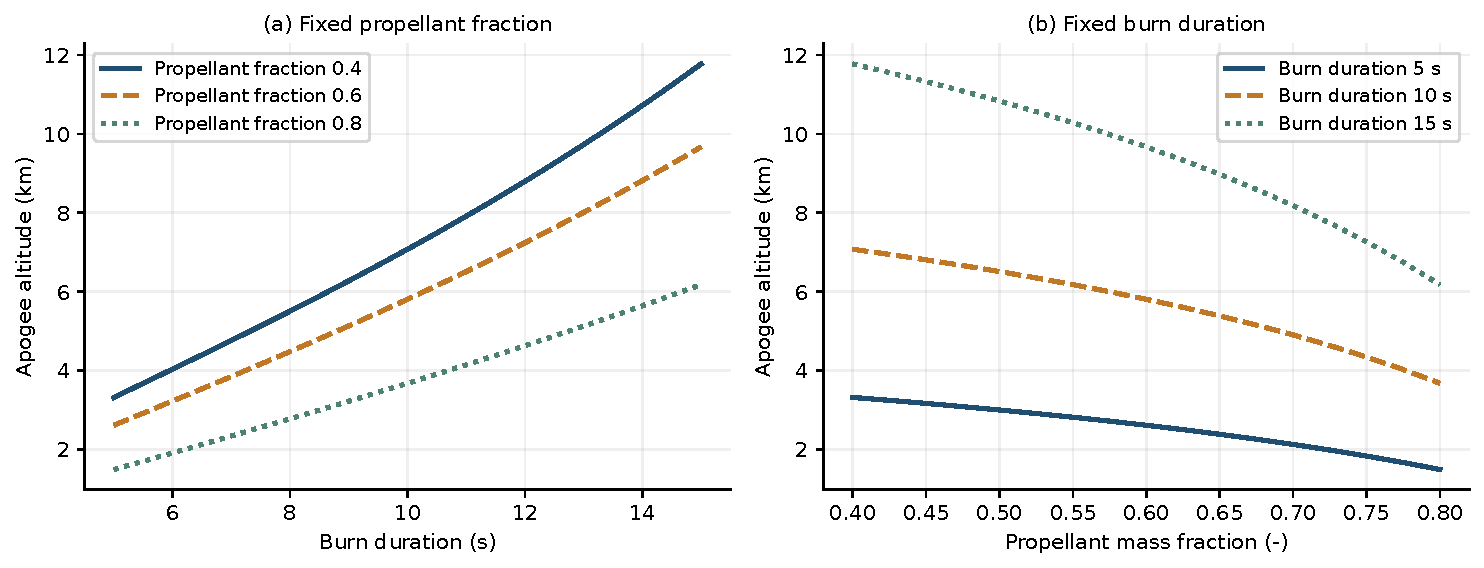
\includegraphics[width=\linewidth]{figures/parameter_slices.pdf}
\caption{Controlled atmospheric sensitivity comparisons. (a) Burn-duration sweeps at three fixed propellant fractions. (b) Fraction sweeps at three fixed burn durations. All curves use $\Delta t=0.125$ s, fixed thrust and fixed dry mass; line styles distinguish cases in grayscale.}
\label{fig:slices}
\end{figure}

\subsection{Combined Effects and Atmospheric Drag}
Figure~\ref{fig:maps} shows the joint dependence. The largest sampled atmospheric apogee is $11771.92$ m at $(15\,\mathrm{s},0.40)$; the smallest is $1491.70$ m at $(5\,\mathrm{s},0.80)$. Both occur on the study boundary. There is no interior maximum among the sampled grid points. This is a statement about the selected grid and constraints, not a proof of a global continuous optimum or a recommendation for a realizable motor.

\begin{figure}[htbp]
\centering
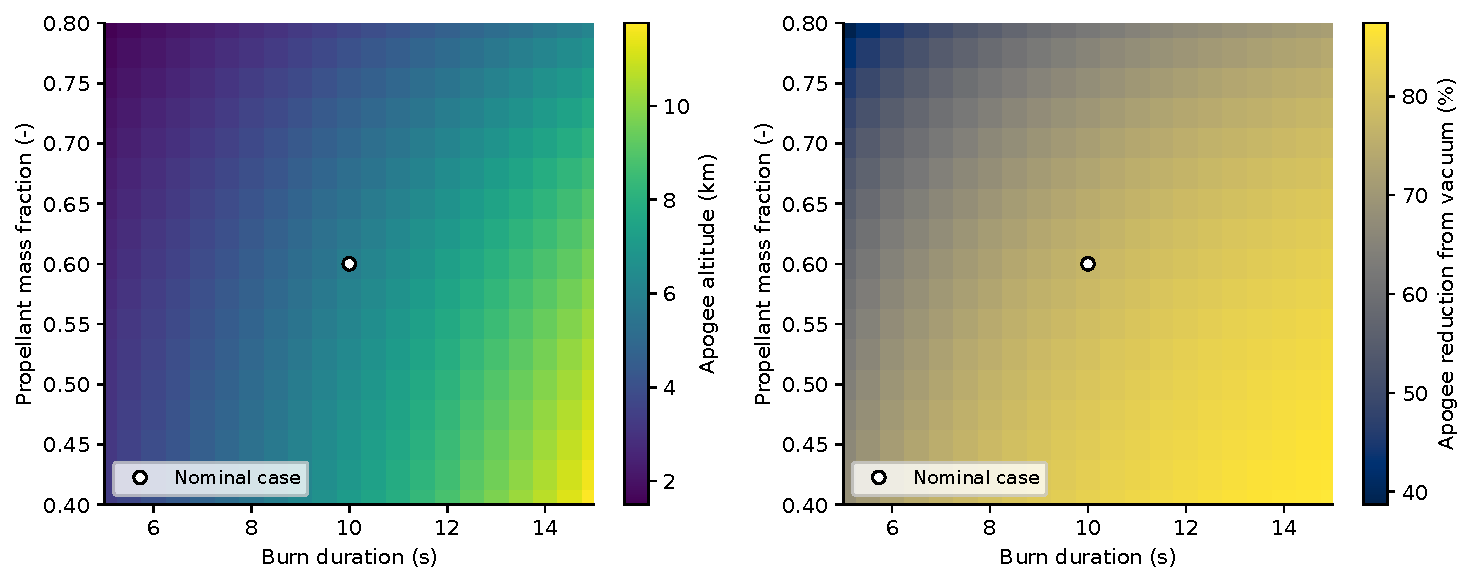
\includegraphics[width=\linewidth]{figures/parameter_maps.pdf}
\caption{The 357-case design grid. Left: atmospheric apogee. Right: relative altitude penalty from Eq.~\eqref{eq:drag-penalty}. White circles locate the nominal case. Colored cells represent computed samples, not additional simulations between samples.}
\label{fig:maps}
\end{figure}

For the nominal configuration, removing drag raises the modeled apogee from $5806.87$ to $25324.08$ m, giving $\Delta h_D=19517.22$ m and $P_D=77.07\%$. Over the full grid, $P_D$ ranges from $38.68\%$ to $87.41\%$. The relative drag penalty increases with burn duration at each sampled fraction and decreases with fraction at each sampled burn duration. Higher-performing vacuum configurations lose a larger fraction of their potential altitude to drag in this model.

The strong loss is consistent with quadratic aerodynamic resistance during high-speed ascent. The exponential atmosphere weakens drag at higher altitude, but does not eliminate its accumulated effect. Figure~\ref{fig:drag-results} compares the two models directly, while Table~\ref{tab:engineering-results} gives representative values. Absolute penalties and all other grid values are available in \texttt{data/engineering\_results.csv}.

\begin{figure}[htbp]
\centering
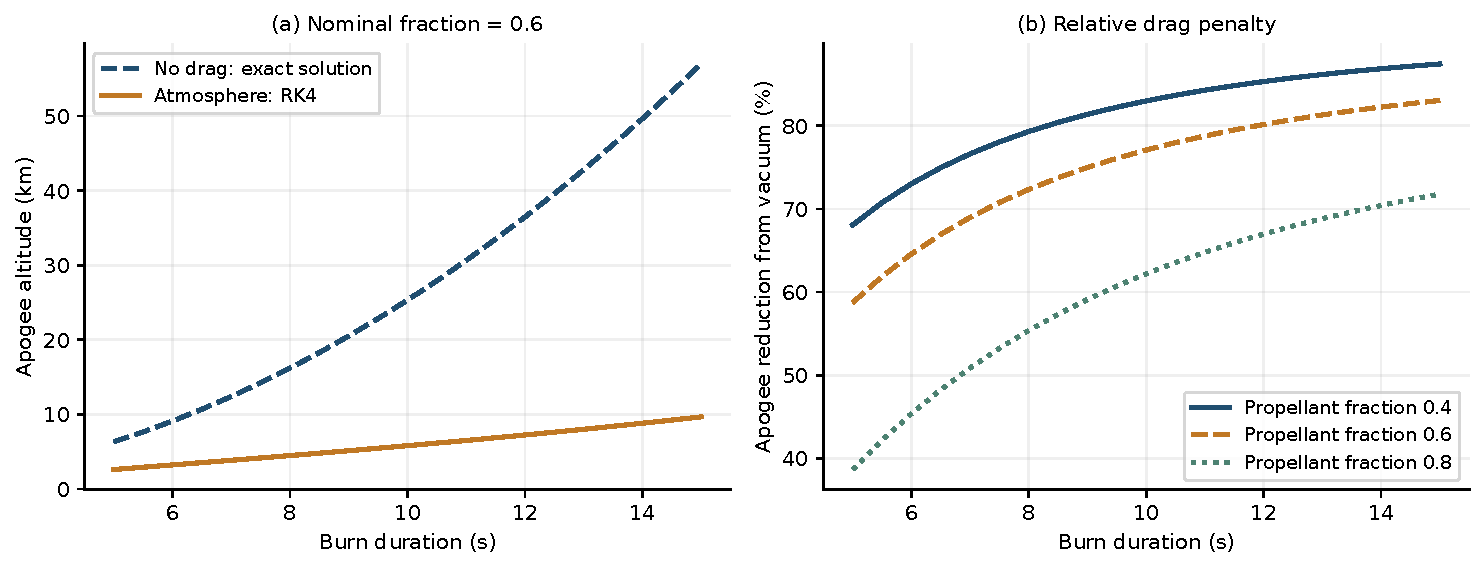
\includegraphics[width=\linewidth]{figures/drag_comparison.pdf}
\caption{Atmospheric drag penalty. (a) Exact vacuum and numerical atmospheric apogees at $\phi=0.60$. (b) Relative reduction from the vacuum apogee for three fractions. Both models use the same constant gravity and vehicle parameters.}
\label{fig:drag-results}
\end{figure}

\begin{table}[htbp]
\centering
\caption{Representative configurations from the executed grid. Atmospheric quantities use $\Delta t=0.125$ s; vacuum apogees are analytical. Values are rounded for presentation.}
\label{tab:engineering-results}
\small
\begin{tabular}{rrrrrr}
\toprule
$t_{\mathrm{burn}}$ (s) & $\phi$ & $h_{\mathrm{ap,atm}}$ (m) & $t_{\mathrm{ap,atm}}$ (s) & $h_{\mathrm{ap,vac}}$ (m) & $P_D$ (\%)\\
\midrule
\inputrows{data/results_table.tex}
\bottomrule
\end{tabular}
\end{table}

\subsection{Engineering Interpretation and Model Limits}
Within the stated family, longer burns and lower propellant fractions produce greater apogee, while drag removes a substantial fraction of the corresponding vacuum altitude. The two design variables cannot be interpreted independently of the constraints: the implied exhaust velocity varies from $156.25$ to $2812.50$ m/s across the grid. A practical motor comparison would need a specified impulse or exhaust-velocity constraint and a compatible thrust/mass-flow law. Those are different studies from the fixed-thrust question answered here.

The parameters are illustrative rather than fitted to a specific vehicle. Constant $C_d$ neglects Mach and Reynolds-number dependence; vertical motion neglects wind, attitude, and lift; constant $g$ and an exponential atmosphere simplify the environment. The largest vacuum apogee is $93.52$ km, where constant gravity is particularly limiting. Vacuum trajectories here are controlled mathematical comparisons, not realistic high-altitude flight forecasts. Numerical convergence and exact-solution tests establish evidence for solving the specified equations; they do not quantify uncertainty in these physical assumptions. No experimental validation or global motor optimization is claimed.

\section{Contributions}
The group worked collaboratively, with each member contributing approximately 25\% of the original project work. The roles reported by the group are summarized below. Additional AI assistance with the calculations, Results section, and revisions is described in the Acknowledgments.
\begin{itemize}
\item \textbf{Maria Dalton (25\%):} Maria explained how the rocket's motion could be formulated as an initial value problem, connecting the known launch conditions to the equations for altitude, velocity, and mass. She also developed the justification for choosing RK4 by discussing its accuracy, stability, and computational cost. For the implementation, Maria worked on the initial Python solver and the logic for switching from powered flight to coasting at burnout. Her work connected the mathematical model to the numerical time-stepping procedure used to calculate the trajectory and apogee.

\item \textbf{Morgan Waller (25\%):} Morgan helped frame the main engineering question about how burn duration and propellant mass fraction affect apogee. For the method section, Morgan developed the discussion of RK4's error and stability properties, including the distinction between the one-step error and the accumulated global error. Morgan also worked on the simulation-parameter evaluation, comparing time-step choices in the powered and coast phases. This work focused on balancing numerical accuracy with computational cost and explaining why a stable time step must also be checked for accuracy.

\item \textbf{Yogeshwari Kant (25\%):} Yogeshwari defined the mathematical functions and parameters used in the rocket model, including the thrust profile, mass depletion, atmospheric density, and aerodynamic drag. She also wrote the algorithmic summary describing how the solver advances the state, handles burnout, and detects apogee. For the convergence study, Yogeshwari worked on the time-step refinement procedure and the analysis of the resulting errors. Her contribution helped explain how a log-log error plot and observed convergence orders can be used to compare the implementation with RK4's expected fourth-order behavior.

\item \textbf{Justin Chiang (25\%):} Justin explained why numerical integration is useful for the coupled, nonlinear rocket equations. He developed the Taylor-series foundation of RK4 and the explanations of its four intermediate slopes and weighted update. For the independent validation, Justin worked on the constant-mass, zero-drag ballistic benchmark and the comparison between numerical trajectories and the exact kinematic solution. This provided a check beyond convergence against a refined numerical result. Justin also prepared the original reproducibility instructions, contribution descriptions, and AI acknowledgment, documenting how the work was organized and how the calculations could be repeated.
\end{itemize}

\section{Reproducibility}
\textbf{Code repository:}\par
\noindent\repositorylink\par
\vspace{\baselineskip}

The package separates the numerical solver, verification experiments, engineering parameter study, and plotting style. Install the pinned dependencies in \texttt{requirements.txt}, then run \texttt{python reproduce.py}. The command executes seven automated tests, all five experiment scripts, and PDF compilation when a local LaTeX installation is available. \lstinline[basicstyle=\ttfamily\normalsize]|python reproduce.py --skip-latex| regenerates all numerical results without a TeX installation. All outputs are written relative to the script directory; no external time-integration solver is used.

The \texttt{data/} directory contains raw trajectory and convergence CSV files, all 25 step-pair comparisons, all 357 engineering cases, diagnostic JSON, the generated Results table, an environment record, and an execution log. Figures are exported in vector PDF and raster PNG formats. Appendix~\ref{app:files} maps scripts to outputs. Numerical differences at the last few floating-point digits may occur across platforms.

For Overleaf, upload the entire project ZIP and select \texttt{main.tex} with pdfLaTeX. The report reads its solver listing from \texttt{rocket\_solver.py} and its Results table from \texttt{data/results\_table.tex}; these files must accompany the figures. Python is not executed by Overleaf. The README gives GitHub upload and local reproduction instructions.

\section{Acknowledgments}
We first brainstormed our project idea as a group and then used ChatGPT to check whether the idea and its assumptions were reasonable. After writing an initial draft, we asked AI to review it and suggest revisions. We followed a similar process for the code: we first attempted to write it ourselves, then used AI to review the implementation, identify errors, and suggest adjustments. We also asked AI for explanations and guidance when we were stuck or unsure how to proceed.

AI assistance included developing additional verification checks, running the parameter studies, generating figures, and helping interpret the results. Finally, we gave the full document to AI for an overall review, including checking technical consistency, organizing the formatting, correcting grammar, and rephrasing unclear sentences. We reviewed the suggested changes and checked the revised equations, code, and results before including them in the report.

\clearpage
\appendix
\section{Supporting Derivations}
\label{app:derivation}
\subsection{Nonlinear Taylor Matching for RK4}
Within one phase the three-state model is autonomous: $u'=F(u)$. Let $J=F'(u)$, $F''$ denote its bilinear second derivative, and $F'''$ its trilinear third derivative, all evaluated at the exact initial state. Successive differentiation gives
\begin{align*}
 u'&=F,\qquad u''=JF,\\
 u'''&=F''(F,F)+J^2F,\\
 u^{(4)}&=F'''(F,F,F)+3F''(F,JF)+JF''(F,F)+J^3F.
\end{align*}
The exact expansion is therefore
\begin{align*}
 u(t+\Delta t)=u
 &+\Delta t F+\frac{\Delta t^2}{2}JF
 +\frac{\Delta t^3}{6}\{F''(F,F)+J^2F\}\\
 &+\frac{\Delta t^4}{24}\{F'''(F,F,F)+3F''(F,JF)+JF''(F,F)+J^3F\}
 +O(\Delta t^5).
\end{align*}
Expanding each stage $F(u+\delta)=F+J\delta+F''(\delta,\delta)/2+F'''(\delta,\delta,\delta)/6+\cdots$ and substituting recursively gives the RK coefficients for these terms:
\begin{center}
\begin{tabular}{lll}
\toprule
Derivative term & RK coefficient & Exact coefficient\\
\midrule
$F$ & $b^T\mathbf{1}$ & $1$\\
$JF$ & $b^Tc$ & $1/2$\\
$F''(F,F)$ & $b^Tc^2/2$ & $1/6$\\
$J^2F$ & $b^TBc$ & $1/6$\\
$F'''(F,F,F)$ & $b^Tc^3/6$ & $1/24$\\
$F''(F,JF)$ & $b^TCBc$ & $1/8$\\
$JF''(F,F)$ & $b^TBc^2/2$ & $1/24$\\
$J^3F$ & $b^TB^2c$ & $1/24$\\
\bottomrule
\end{tabular}
\end{center}
Here $B,b,c,C$ are those in Section~2. Inserting the classical RK4 coefficients satisfies each equality and establishes fourth-order matching for nonlinear systems, not merely the linear test equation. This is an independent expansion supplementing the lecture presentation. The derivation applies separately on each side of burnout; it does not assume a differentiable thrust function across the switch.

\subsection{Exact Powered-Plus-Coast Vacuum Apogee}
\label{app:vacuum}
Let $q=(m_0-m_{\mathrm{dry}})/t_{\mathrm{burn}}>0$ and set $C_d=0$. With $h(0)=v(0)=0$, direct integration gives
\begin{align*}
 v(t)&=\frac{T_0}{q}\ln\frac{m_0}{m_0-qt}-gt,\\
 h(t)&=\frac{T_0}{q^2}\left[qt-(m_0-qt)\ln\frac{m_0}{m_0-qt}\right]-\frac12gt^2.
\end{align*}
At $t=t_{\mathrm{burn}}$, denote these values by $h_b,v_b$. In coast, for $s=t-t_{\mathrm{burn}}$, $v=v_b-gs$ and $h=h_b+v_bs-gs^2/2$. If $v_b>0$ and $g>0$, then
\[
 t_{\mathrm{ap,vac}}=t_{\mathrm{burn}}+\frac{v_b}{g},\qquad
 h_{\mathrm{ap,vac}}=h_b+\frac{v_b^2}{2g}.
\]
All study configurations lift off immediately and have $v_b>0$. At fixed $\phi$ and dry mass, let $m_p=m_0-m_{\mathrm{dry}}$ and $L=\ln(m_0/m_{\mathrm{dry}})$, both independent of burn duration. Substituting $q=m_p/t_{\mathrm{burn}}$ gives
\[
 h_{\mathrm{ap,vac}}=t_{\mathrm{burn}}^2
 \left\{\frac{T_0}{m_p^2}(m_p-m_{\mathrm{dry}}L)-\frac{g}{2}
 +\frac{1}{2g}\left(\frac{T_0L}{m_p}-g\right)^2\right\}.
\]
Thus the vacuum altitude scales quadratically with duration under these particular constraints. The bracket has units of acceleration, so multiplication by time squared gives altitude. This formula is used as an independent check of the numerical solver, including the powered/coast transition and apogee localization.

\subsection{Signs and Dimensions}
The positive axis points upward. Thrust is positive during burn; gravity contributes $-g$; and $-\rho C_d A v|v|/2$ opposes either direction of motion. Density has units kg/m$^3$, so $\rho A v|v|$ has units N and $D/m$ has units m/s$^2$. The exponent $h/H$ and mass ratio inside the logarithm are dimensionless. The mass-flow rate $q$ has units kg/s, $T_0/q$ has units m/s, and all analytical solutions satisfy $h(0)=v(0)=0$ and $m(0)=m_0$.

\section{Reproducibility File Map}
\label{app:files}
\small
\begin{tabular}{>{\raggedright\arraybackslash}p{.31\linewidth}>{\raggedright\arraybackslash}p{.63\linewidth}}
\toprule
File & Purpose and principal outputs\\
\midrule
\texttt{rocket\_solver.py} & Parameters, signed-drag derivative, RK4 stages, burnout alignment and apogee event.\\
\texttt{plot\_trajectory.py} & Nominal trajectory CSV; altitude, velocity, mass and combined trajectory figures.\\
\texttt{convergence\_study.py} & Reference refinement, apogee-error CSV, adjacent orders, fitted convergence figure.\\
\texttt{validation.py} & Independent ballistic and powered vacuum solutions; validation CSV files and figure.\\
\texttt{parameter\_evaluation.py} & All 25 phase-step pairs, RHS cost counts and nominal diagnostics.\\
\texttt{engineering\_results.py} & All 357 configurations, three-level refinement, exact-vacuum comparisons, three engineering figures, summary JSON and report table.\\
\texttt{plot\_style.py} & Common plotting appearance; vector PDF and raster PNG export.\\
\texttt{test\_solver.py} & Seven tests: ballistic limit, powered order, nonaligned burnout, drag coefficient/sign/density, rejected failures, vacuum apogee, and evaluation count.\\
\texttt{reproduce.py} & Runs tests and experiments; records environment and execution log; compiles report when available.\\
\texttt{requirements.txt} & Pinned NumPy and Matplotlib versions used for the executed study.\\
\texttt{README.md} & Setup, model assumptions, commands, expected outputs, and GitHub/Overleaf instructions.\\
\texttt{data/}, \texttt{figures/} & Generated numerical evidence and figures referenced in the report.\\
\bottomrule
\end{tabular}
\normalsize


\clearpage
\section{Complete Core Solver}
\label{app:code}
The listing below is read directly from the executed source file, preventing a separately maintained code transcription. The experiment and test scripts accompany it in the repository. 
\subsection{Parameters, Derivatives, and RK4 Step}
\lstinputlisting[basicstyle=\ttfamily\fontsize{7}{8}\selectfont,firstline=1,lastline=66,caption={Core solver: physical parameters, derivative evaluation, and RK4.},label={lst:solver}]{rocket_solver.py}
\clearpage
\subsection{Apogee Localization and Time Marching}
\lstinputlisting[basicstyle=\ttfamily\fontsize{7}{8}\selectfont,firstline=67,firstnumber=67]{rocket_solver.py}

\end{document}
